%=============================================================================%
% Author: 	John Joseph Valletta (modified by Richard B Sherley)
% Date: 	07/11/2018 (Modified 25/02/2020)
% Title: 	Fews slides for generalised linear model workshop
%=============================================================================%

%=============================================================================%
% Preamble
%=============================================================================%
% Libraries
\ifdefined\handoutmode
    \documentclass[pdf,handout]{beamer}
\else
    \documentclass[pdf]{beamer}
\fi
\usepackage[export]{adjustbox}
\usepackage{framed}
\usepackage{color}
\definecolor{dkgreen}{rgb}{0,0.6,0}
\definecolor{gray}{rgb}{0.5,0.5,0.5}
\definecolor{mauve}{rgb}{0.58,0,0.82}
\definecolor{deepblue}{rgb}{0,0,0.5}
\definecolor{deepred}{rgb}{0.6,0,0}
\definecolor{deepgreen}{rgb}{0,0.5,0}
\definecolor{lightgray}{rgb}{0.92,0.92,0.92}
\usepackage{listings} % to insert code
\usepackage{textpos} % textblock
\usepackage{verbatim}
\usepackage{longtable}
\usepackage{hyperref}
\hypersetup{colorlinks=true, urlcolor=blue, linkcolor=white} 

% Listing set up
\lstdefinestyle{R}{
language=R,                     % the language of the code
basicstyle=\scriptsize\ttfamily,% the size of the fonts that are used for the code
numbers=left,                   % where to put the line-numbers
numberstyle=\tiny\color{white},  % the style that is used for the line-numbers
stepnumber=1,                   % the step between two line-numbers. If it's 1, each line
                          		% will be numbered
numbersep=5pt,                  % how far the line-numbers are from the code
backgroundcolor=\color{lightgray},  % choose the background color. You must add \usepackage{color}
showspaces=false,               % show spaces adding particular underscores
showstringspaces=false,         % underline spaces within strings
showtabs=false,                 % show tabs within strings adding particular underscores
frame=lines,%single,                   % adds a frame around the code
rulecolor=\color{black},        % if not set, the frame-color may be changed on line-breaks within not-black text (e.g. commens (green here))
tabsize=2,                      % sets default tabsize to 2 spaces
captionpos=b,                   % sets the caption-position to bottom
breaklines=true,                % sets automatic line breaking
breakatwhitespace=false,        % sets if automatic breaks should only happen at whitespace
title=\lstname,                 % show the filename of files included with \lstinputlisting;
                          		% also try caption instead of title
keywordstyle=\color{blue},      % keyword style
commentstyle=\color{dkgreen},   % comment style
stringstyle=\color{mauve},      % string literal style
escapeinside={\%*}{*)},         % if you want to add a comment within your code
morekeywords={}            		% if you want to add more keywords to the set
}

% Presentation configuration
\mode<presentation>{\usetheme{Madrid}}
\definecolor{tealblue}{rgb}{0, 0.3, 0.6}
\usecolortheme[named=tealblue]{structure}
\useinnertheme{circles} % circles, rectanges, rounded, inmargin
\usefonttheme[onlymath]{serif} % makes math fonts like the usual LaTeX ones
\setbeamercovered{transparent=4} % transparent
\setbeamertemplate{caption}{\raggedright\insertcaption\par} % Remove the word "Figure" from caption %\setbeamertemplate{caption}[default]
\setbeamertemplate{navigation symbols}{} % don't put navigation tools at the bottom (alternatively \beamertemplatenavigationsymbolsempty)
\graphicspath{ {./img/} }

% Titlepage
\title[GLMs in R]{Generalised linear models in R}
%\subtitle{Built-in data types}
\author{Richard B. Sherley}
\date[March 2020]{March 2020}
\institute[]{University of Exeter, Penryn Campus, UK}
\titlegraphic{
\hfill

\includegraphics[width=\textwidth, keepaspectratio]{logo.jpg}}

%=============================================================================%
%=============================================================================%
% Start of Document
%=============================================================================%
%=============================================================================%
\begin{document}

%=============================================================================%
%=============================================================================%
\begin{frame}
\titlepage
\end{frame}

%=============================================================================%
%=============================================================================%
\begin{frame}{Reminder}
Extensive notes, handouts of these slides, and data files for the practicals are available at: 
\href{https://exeter-data-analytics.github.io/StatModelling/}{https://exeter-data-analytics.github.io/StatModelling/}
\end{frame}
%=============================================================================%
%=============================================================================%
\begin{frame}{Recap: Linear regression}

\textbf{Assumptions}:

\begin{enumerate}\addtolength{\itemsep}{1\baselineskip}
    \item A \textbf{linear} mean function is relevant.
    \item Variances are equal across all predicted values of the response (\textbf{homoscedatic}).
    \item Errors are \textbf{normally} distributed. 
    \item Samples collected at \textbf{random}.
    \item Errors are \textbf{independent}.
\end{enumerate}

\end{frame}

%=============================================================================%
%=============================================================================%
\begin{frame}{Generalised linear models (GLMs)}

\begin{enumerate}\addtolength{\itemsep}{2\baselineskip}
    \item A linear mean (including any explanatory variables you want to)\\ i.e $\beta_0 + \beta_1X_1 + \ldots + \beta_pX_p$
    \item A \textbf{link function} (like an ``internal" transformation).
    \item An \textbf{error structure}.\\ So far we assumed normality $\epsilon \sim \mathcal{N}(0,\sigma^2)$
\end{enumerate}

\end{frame}

%=============================================================================%
%=============================================================================%
\begin{frame}{Link functions}

\textbf{Links} your \textbf{mean} function to the \textit{scale} of the \textbf{observed data} e.g.

$$
E(Y) = g^{-1}\left(\beta_0 + \beta_1 X\right)
$$

\vfill

\begin{itemize}\addtolength{\itemsep}{2\baselineskip}
    \item $\mathbb{E}(Y)$ is the \textbf{expected value} (i.e. mean of $Y$).
    \item The function $g(\cdot)$ is known as the \textbf{link function}, and $g^{-1}(\cdot)$ denotes the \textbf{inverse} of $g(\cdot)$.
\end{itemize}

\end{frame}

%=============================================================================%
%=============================================================================%
\begin{frame}{Simple linear regression is a special case of a GLM}

\begin{enumerate}\addtolength{\itemsep}{2\baselineskip}
    \item<1-> A linear mean: $\beta_0 + \beta_1X_1 + \ldots + \beta_pX_p$
    \item<2-> An \textbf{error structure}: $\epsilon \sim \mathcal{N}(0,\sigma^2)$
    \item<3-> \textbf{Link function}: \textbf{identity}\\
    $\mu = \beta_0 + \beta_1X_1 + \ldots + \beta_pX_p$
\end{enumerate}

\vfill 

\visible<4->{
$$
\begin{aligned}
Y & \sim \mathcal{N}(\mu, \sigma^2) \\
\mu & = \beta_0 + \beta_1X
\end{aligned}
$$
}

\end{frame}

%=============================================================================%
%=============================================================================%
\begin{frame}[fragile]
\frametitle{GLMs in R}


\begin{lstlisting}[style=R]
lm(height ~ weight, data=df)
\end{lstlisting}


Is equivalent to:
\vfill

\begin{lstlisting}[style=R]
glm(height ~ weight, data=df, family=gaussian(link=identity))
\end{lstlisting}

\vfill

\texttt{family} specifies the error structure \textbf{and} link function

\end{frame}

%=============================================================================%
%=============================================================================%
\begin{frame}{Default link functions}

\begin{longtable}[]{c|c}
\textbf{Family} & \textbf{Link}\tabularnewline\hline
\texttt{gaussian} & \textbf{\texttt{identity}}\tabularnewline
\texttt{binomial} & \textbf{\texttt{logit}}, \texttt{probit} or
\texttt{cloglog}\tabularnewline
\texttt{poisson} & \textbf{\texttt{log}}, \texttt{identity} or
\texttt{sqrt}\tabularnewline
\texttt{Gamma} & \textbf{\texttt{inverse}}, \texttt{identity} or
\texttt{log}\tabularnewline
\texttt{inverse.gaussian} & \textbf{\texttt{1/mu\^{}2}}\tabularnewline
\texttt{quasi} & user-defined\tabularnewline
\texttt{quasibinomial} & \textbf{\texttt{logit}}\tabularnewline
\texttt{quasipoisson} & \textbf{\texttt{log}}\tabularnewline
\end{longtable}

\end{frame}

%=============================================================================%
%=============================================================================%
\begin{frame}{Poisson regression}

Count data is \textbf{discrete} and \textbf{non-negative}

\begin{figure}
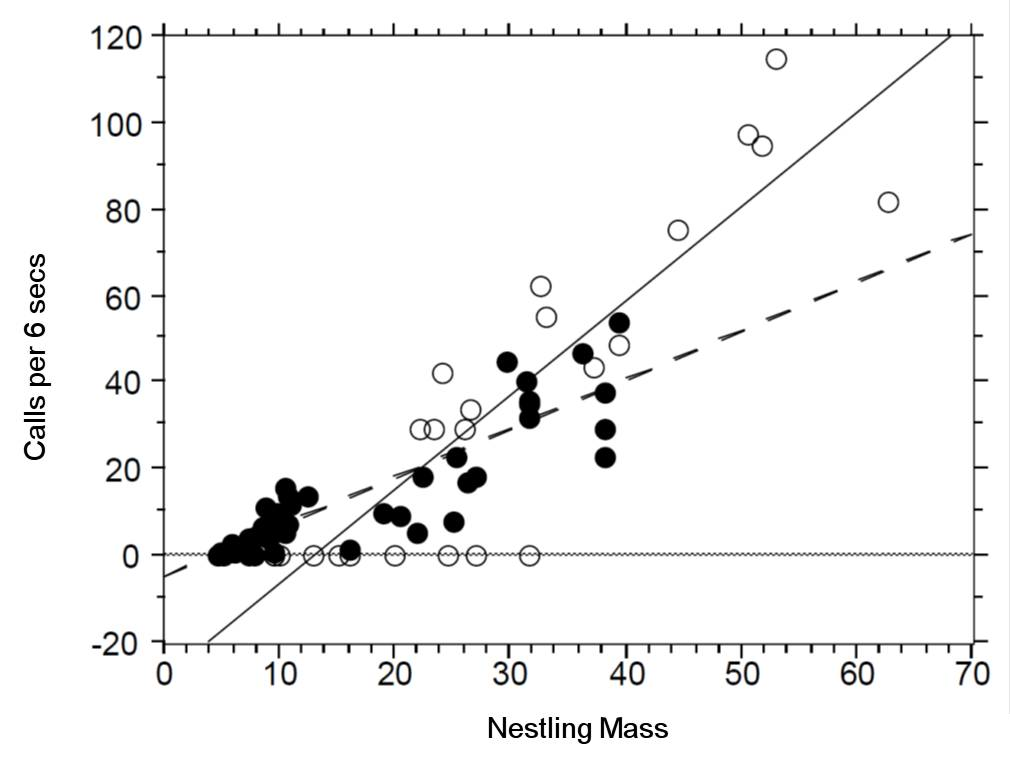
\includegraphics[width=.5\textwidth]{cuckooanalysis.png}
\end{figure}

\vspace{-.5cm}

\visible<2->{
$$
\begin{aligned}
Y & \sim \mathcal{N}(\mu, \sigma^2) &&& Y & \sim \mathcal{P}ois(\mu) \\
\mu & = \beta_0 + \beta_1X &&& \log{\mu} & = \beta_0 + \beta_1X
\end{aligned}
$$}

\end{frame}

%=============================================================================%
%=============================================================================%
\begin{frame}{Poisson distribution}

\begin{itemize}\addtolength{\itemsep}{.5\baselineskip}
    \item \textbf{Discrete} variable, defined on the range $0, 1, \dots, \infty$.
    \item  A single \textbf{rate} parameter $\lambda$, where $\lambda > 0$.
    \item \textbf{Mean} = $\lambda$  
    \item \textbf{Variance} = $\lambda$
\end{itemize}

\begin{figure}
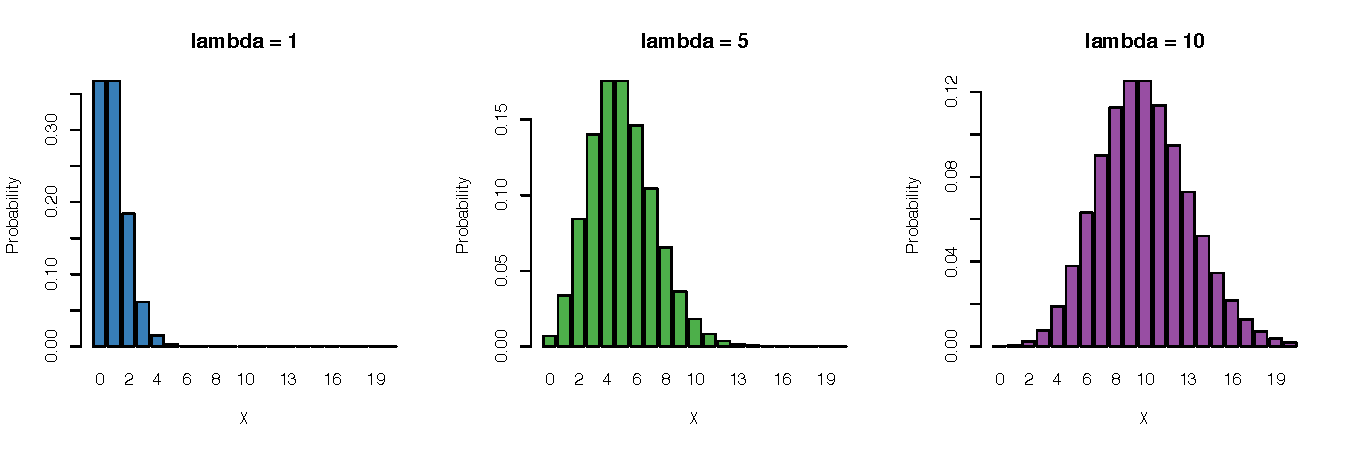
\includegraphics[width=.75\textwidth]{poissondist.pdf}
\end{figure}

\end{frame}

%=============================================================================%
%=============================================================================%
\begin{frame}[fragile]
\frametitle{Poisson regression}

$$
\begin{aligned}
Y & \sim \mathcal{P}ois(\lambda) \\
\log{\lambda} & = \beta_0 + \beta_1X
\end{aligned}
$$

\vfill
Using the rules of logarithm (i.e $\log{\lambda} = k$, then $\lambda = e^k$):

$$
\begin{aligned}
\log{\lambda} & = \beta_0 + \beta_1X \\
\lambda & = e^{\beta_0 + \beta_1X }
\end{aligned}
$$

\vfill
Thus we are effectively modelling the observed counts using an exponential distribution

\begin{lstlisting}[style=R]
glm(outcome ~ explanatory, data=df, family=poisson(link=log))
\end{lstlisting}


\end{frame}

%=============================================================================%
%=============================================================================%
\begin{frame}{Cuckoo data}

\begin{figure}
\includegraphics<1>[width=.75\textwidth]{cuckooanalysis.png}
\includegraphics<2>[width=.65\textwidth]{cuckooafter.png}
\end{figure}

\end{frame}

%=============================================================================%
%=============================================================================%
\begin{frame}{Logistic regression}

Consider a \textbf{categorical} response variable with two levels (e.g pass/fail). 
These type of \textbf{binary} data are assumed to be \textbf{Bernoulli} distributed:

$$
Y \sim \mathcal{B}ern(p)
$$

\begin{itemize}\addtolength{\itemsep}{.25\baselineskip}
    \item A \textbf{probability} parameter $p$, where $0 < p < 1$.
    \item \textbf{Mean} = $p$  
    \item \textbf{Variance} = $p(1 - p)$
\end{itemize}

\begin{figure}
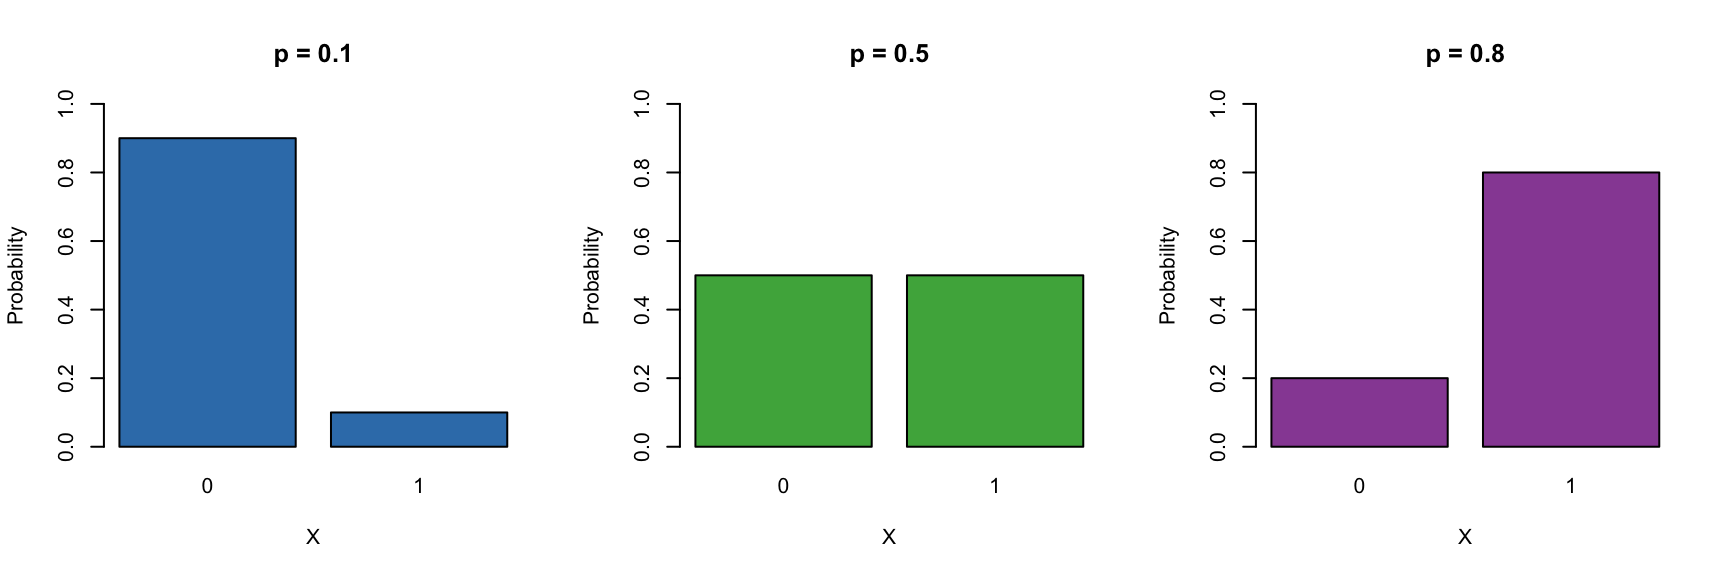
\includegraphics[width=.9\textwidth]{berndist.png}
\end{figure}

\end{frame}

%=============================================================================%
%=============================================================================%
\begin{frame}{Logistic regression}

$$
\begin{aligned}
Y & \sim \mathcal{N}(\mu, \sigma^2) &&& Y  \sim \mathcal{P}ois(\lambda) &&&&&& Y  \sim \mathcal{B}ern(p)\\
\mu & = \beta_0 + \beta_1X &&& \log{\lambda} = \beta_0 + \beta_1X &&&&&& ?? = \beta_0 + \beta_1X
\end{aligned}
$$

\vfill

\visible<2->{
$$
\begin{aligned}
Y  & \sim \mathcal{B}ern(p)\\
\log\left(\frac{p}{1 - p}\right) &  = \beta_0 + \beta_1 X \\
\text{logit}(p) &  = \beta_0 + \beta_1 X
\end{aligned}
$$}

\end{frame}

%=============================================================================%
%=============================================================================%
\begin{frame}[fragile]
\frametitle{Logistic regression}

\scriptsize
$$
\begin{aligned}
\log\left(\frac{p}{1 - p}\right) &  = \beta_0 + \beta_1 X\\
p & = \frac{e^{\beta_0 + \beta_1 X}}{1 + e^{\beta_0 + \beta_1 X}}
\end{aligned}
$$

\normalsize
\vfill

\begin{figure}
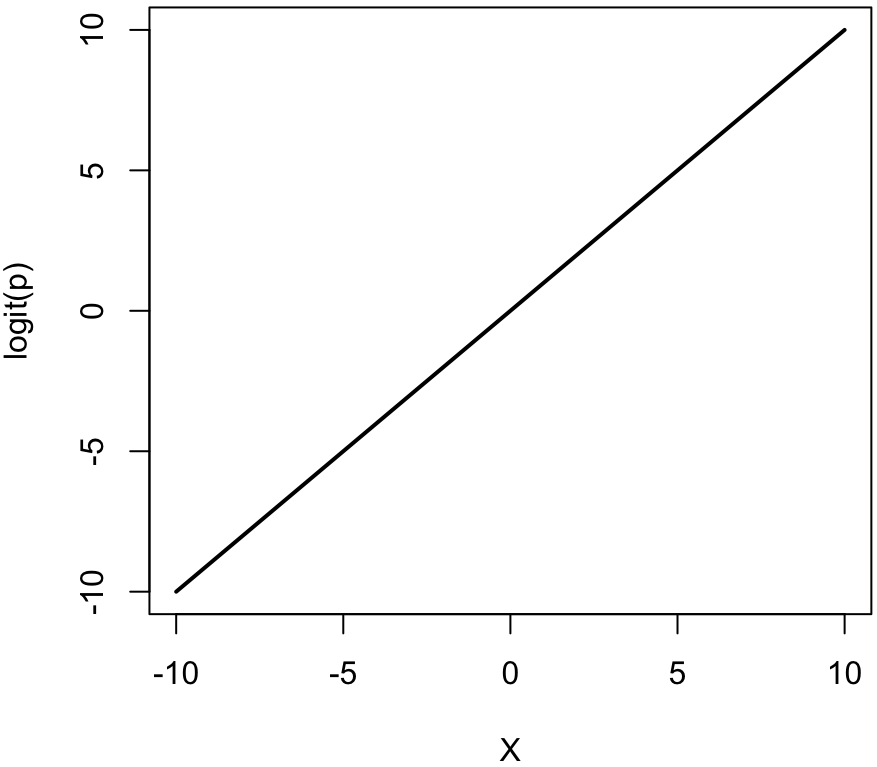
\includegraphics[width=.4\textwidth]{logit.png}
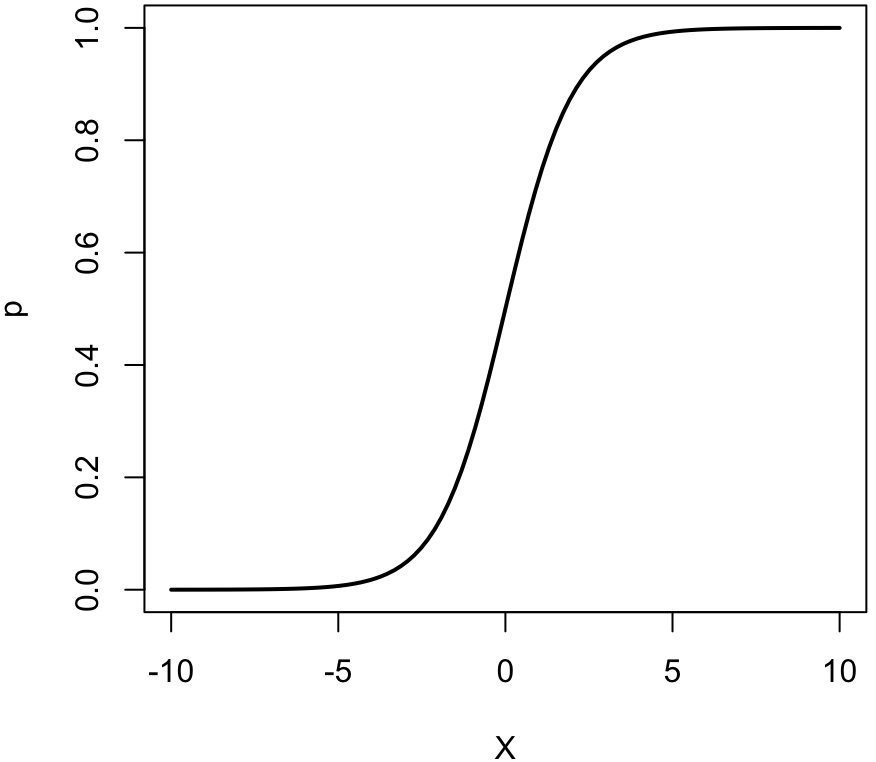
\includegraphics[width=.4\textwidth]{invlogit.png}
\end{figure}

\begin{lstlisting}[style=R]
glm(response ~ explanatory, data=df, family=binomial(link=logit))
\end{lstlisting}

\end{frame}

%=============================================================================%
%=============================================================================%
\begin{frame}{1992 US election survey}

\begin{figure}
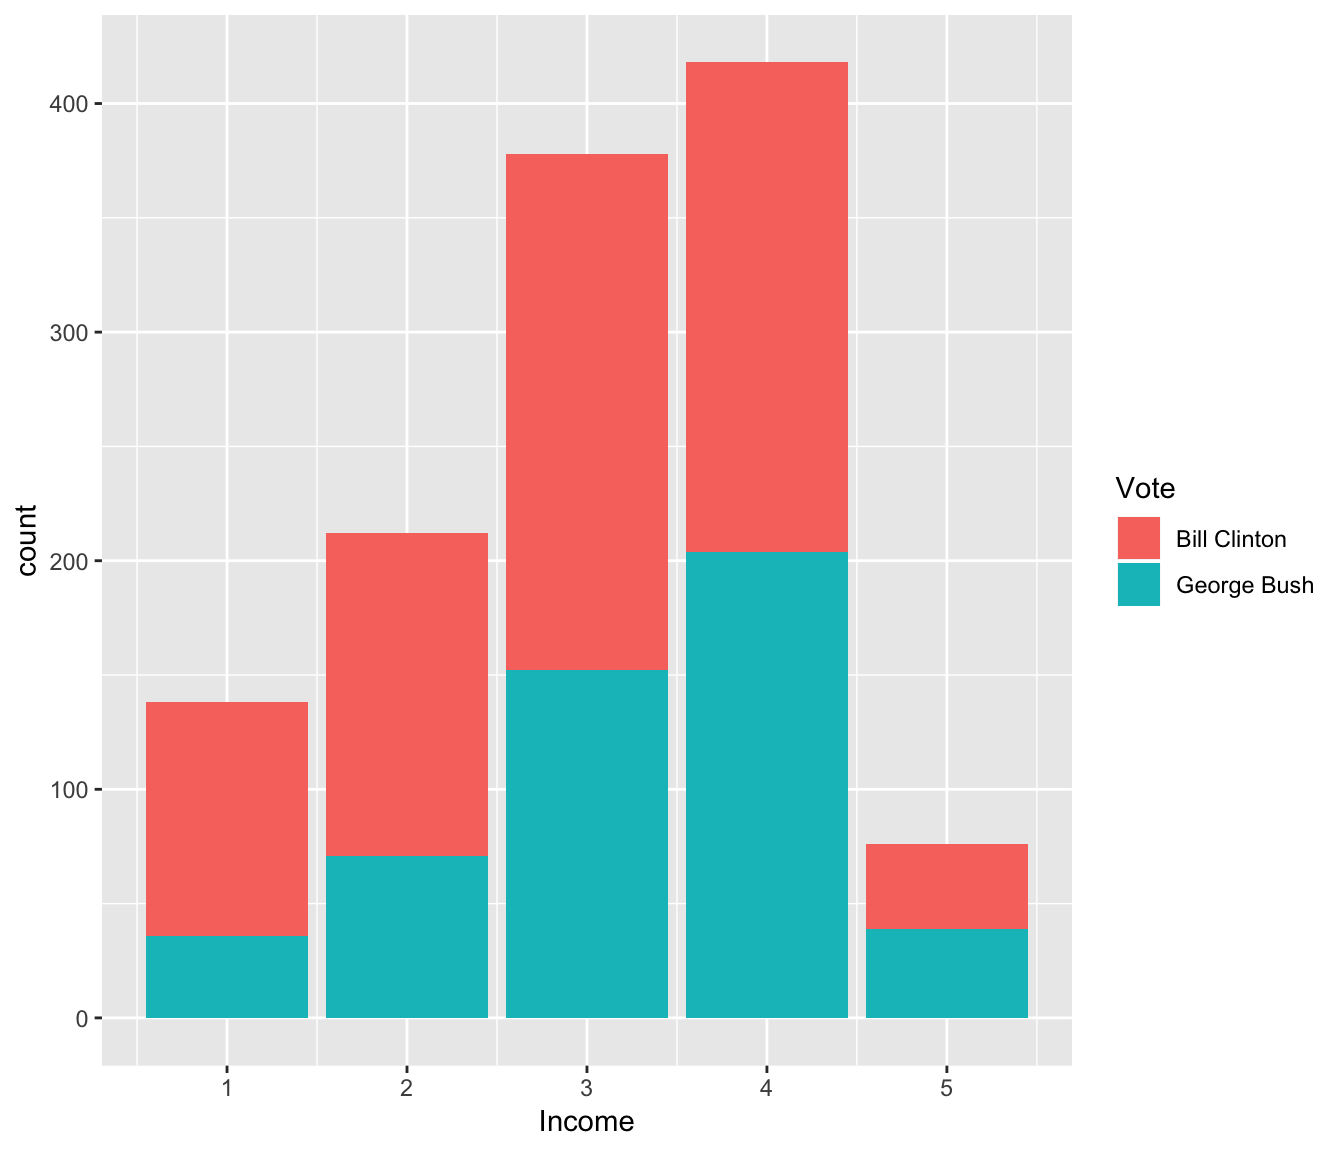
\includegraphics[width=.7\textwidth]{survey.png}
\end{figure}

\end{frame}

%=============================================================================%
%=============================================================================%
\begin{frame}[fragile]
\frametitle{1992 US election survey}

\begin{lstlisting}[style=R]
fit <- glm(Vote ~ Income, data=USA, family=binomial(link=logit))
summary(fit)
\end{lstlisting}

\tiny
\begin{verbatim}
## 
## Call:
## glm(formula = Vote ~ Income, family = binomial(link = logit), 
##     data = USA)
## 
## Deviance Residuals: 
##     Min       1Q   Median       3Q      Max  
## -1.2699  -1.0162  -0.8998   1.2152   1.6199  
## 
## Coefficients:
##             Estimate Std. Error z value Pr(>|z|)    
## (Intercept)  -1.3017     0.1828  -7.122 1.06e-12 ***
## Income        0.3033     0.0551   5.505 3.69e-08 ***
## ---
## Signif. codes:  0 '***' 0.001 '**' 0.01 '*' 0.05 '.' 0.1 ' ' 1
## 
## (Dispersion parameter for binomial family taken to be 1)
## 
##     Null deviance: 1655.0  on 1221  degrees of freedom
## Residual deviance: 1623.5  on 1220  degrees of freedom
## AIC: 1627.5
## 
## Number of Fisher Scoring iterations: 4
\end{verbatim}
\normalsize

\end{frame}

%=============================================================================%
%=============================================================================%
\begin{frame}[fragile]
\frametitle{1992 US election survey}

$$
\begin{aligned}
Y  & \sim \mathcal{B}ern(p)\\
\log\left(\frac{p}{1 - p}\right) &  = \beta_0 + \beta_1 X
\end{aligned}
$$

\begin{itemize}
\item \texttt{`(Intercept)`} = $\beta_0$ = -1.3
\item \texttt{`Income`} = $\beta_1$ = 0.303
\end{itemize}

It is common to interpret variables according to some \textbf{central tendency} e.g at
the central income category (i.e $X=3$)

$$
\begin{aligned}
P(\mbox{Republican vote at}~X = 3) &= \mbox{logit}^{-1}\left(-1.3 + 0.3 \times 3\right)\\
&= \frac{e^{-1.3 + 0.3 \times 3}}{1 + e^{-1.3 + 0.3 \times 3}}\\
&= 0.48.
\end{aligned}
$$

\end{frame}


%=============================================================================%
%=============================================================================%
% End of Document
%=============================================================================%
%=============================================================================%
\end{document}
